\section{Reconstruction}

The FEC reconstruction service provides a fast and efficient algorithm for grouping scintillator $\it{strips}$ with $\it{hits}$ into multiple $\it{peaks}$ and $\it{clusters}$ within a single sector for each of the FEC modules PCAL, ECIN and ECOU, while leaving cluster matching and particle identification to the Event Builder service.  Within the FEC service, these various elements exist as objects with methods, structures and data members designed for calibration, pattern recognition, diagnostics, and serial output.  For example the service applies run-dependent calibration corrections for conversion of raw FADC and TDC digitized data to energy and time, and also provides formatted output banks used by external services.  Also energy thresholds and cluster identification criteria can be configured to optimize reconstruction efficiency, suppress backgrounds and avoid false or duplicate clusters arising from fluctuations at the fringes of electromagnetic showers. 

\begin{figure}[hbt]
\centering
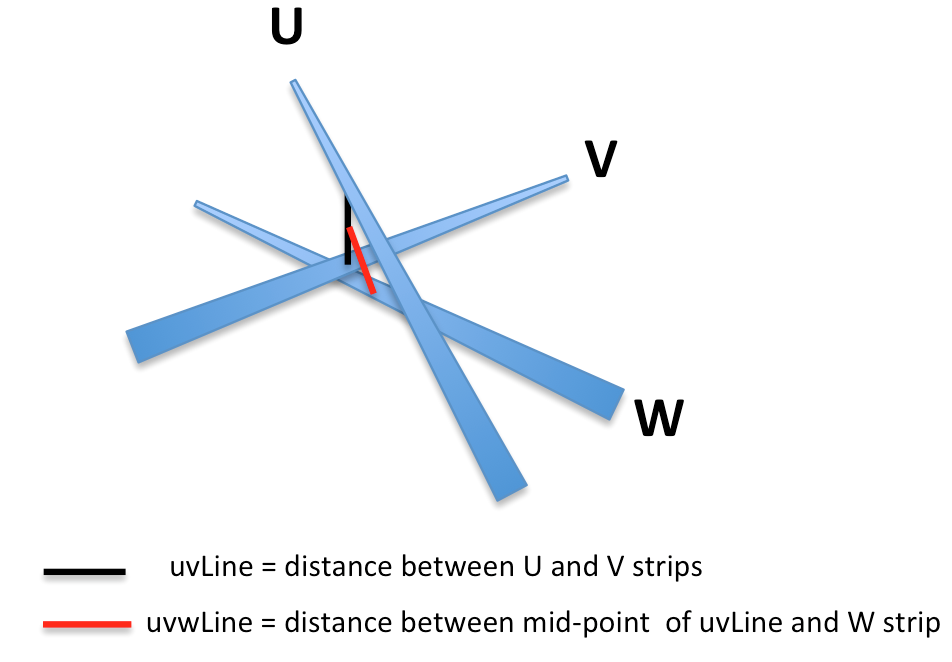
\includegraphics[width=0.95\columnwidth,keepaspectratio]{img/S6_0.png}
\caption{Schematic shows the 3D relationship of the U,V,W peak lines and the metrics used to define the cluster lab-frame coordinates ($x,y,z$).}
\label{fig:S6_0}
\end{figure}

The cluster finding algorithm makes use of the unique geometry and stereo readout features of the FEC. As discussed earlier, each triangular scintillator layer in the FEC lead:scintillator sandwich is transversely divided into strips, with the shortest strip at the corners. The slice direction rotates by $\approx 120^{\circ}$ for each successive layer, providing three $\it{views}$ labeled U, V and W.  For each strip within a view, the layers are optically ganged together into a stack.  Individual PMT readout of each PCAL, ECIN and ECOU stack provides a pulse proportional to the summed energy deposited in the stack.

The algorithm begins by finding collections of contiguous strips having signals above a user-defined threshold for each of the three views. These groupings are called $\it{peaks}$ and their member strips are referred to as $\it{hits}$.  Peak objects may be further subdivided based on the hit energy profile of the groupings.  Each peak object is associated with the one or more stacks of strips that belong to it, and the three-dimensional geometry of each stack is stored along with the peak data.  The service uses this geometry data to determine which collection of peaks belong to $\it{clusters}$. 

\begin{figure}[hbt]
\centering
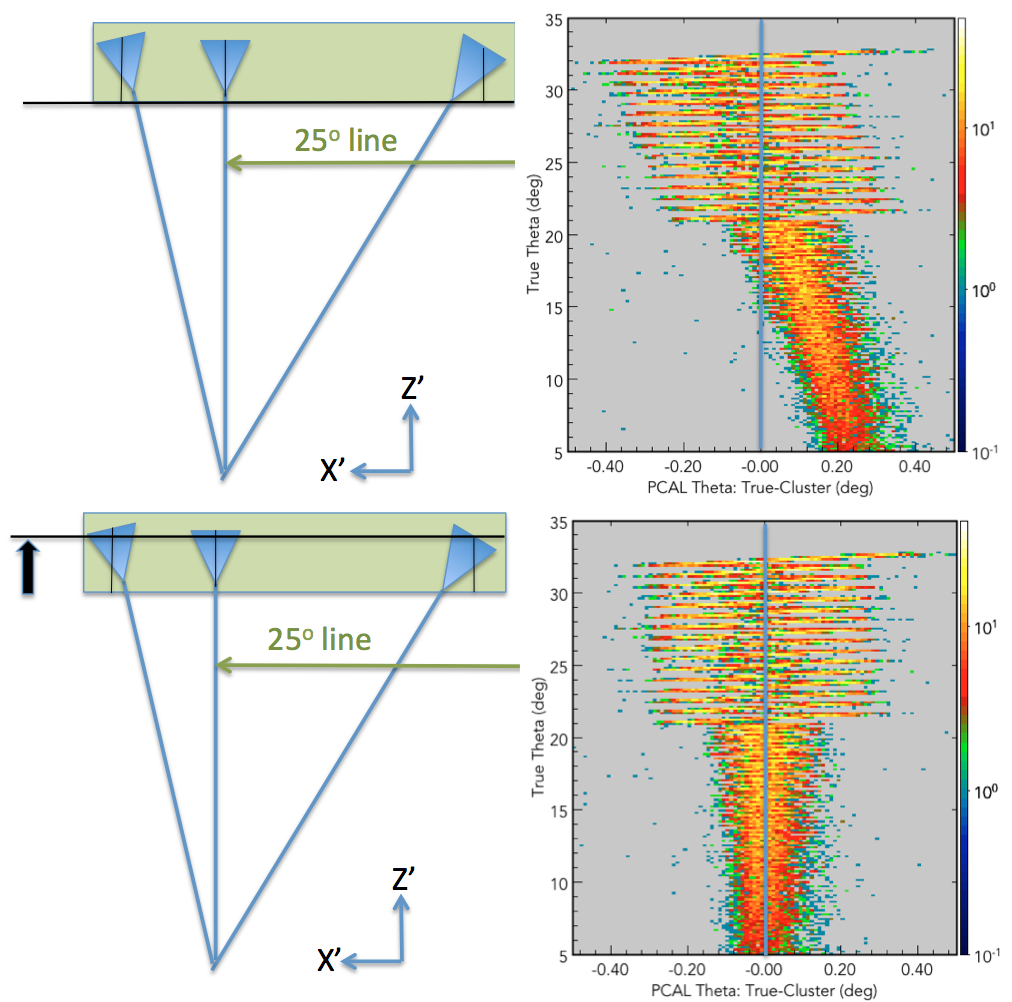
\includegraphics[width=0.95\columnwidth,keepaspectratio]{img/S6_1.png}
\caption{Left: Schematic shows how off-normal tracks with showers peaking at the rear of the calorimeter have a $x'$ projection at the front surface which creates parallax errors for a $z'$ reporting plane at the surface.  Right: GEMC simulation of 2 GeV photons originating at the target demonstrates the error in reconstructed $\theta$ for $z'$ at the first V strip (top) and the fourth V strip (bottom).}
\label{fig:S6_1}
\end{figure}

\subsection {Cluster Position}
The criterion for a cluster requires the spatial intersection of three peaks, one from each of the U, V and W views.  Candidate peaks for a cluster search are based on a user-defined threshold for the summed peak raw energy.  Each peak is represented geometrically as a directed line segment determined by the energy-weighted average of the mid-lines of each member strip.   The degree of intersection of each U,V,W peak triplet is determined by calculating the line of closest distance between a U and V peakline, followed by the line of closest distance between the midpoint of the UV line and the W peakline.  A user-defined cut on this final UV-W distance identifies the cluster, and the midpoint of the UV-W line defines the $x,y,z$ lab-frame coordinates of the cluster (Fig.~\ref{fig:S6_0}).  

Because the calorimeter hodoscope design measures only the transverse ($x',y'$) position of clusters in the local frame (see Fig.~\ref{fig:S6_1}), the $z'$ reporting plane in PCAL must be chosen to coincide with the layer of maximum energy deposition, to avoid parallax errors for tracks that are not normal to the face of the module \cite{nima2018}.  This effect is demonstrated in Fig.~\ref{fig:S6_1} using a GEMC Monte Carlo simulation of 2 GeV photons diverging from the target position along the mid-plane and over the full polar angle $\theta$ range of PCAL.  Using a $z'$ reporting plane at the first V strip (top) clearly introduces a $
\theta$-dependent error in photon angle reconstruction, while moving this plane to the fourth V strip (bottom) minimizes this error.  For the EC module the parallax shift is compensated by the projective geometry that was designed into the scintillators.   

\subsection {Cluster Energy}

Once the cluster is localized, the path from the cluster position to the PMT readout end is calculated for each U,V,W peakline and the peak energies are corrected for scintillator light attenuation.  For isolated clusters the cluster energy is then defined as the sum of the corrected energy from each of the U, V and W peaks that define the cluster.  

More complicated scenarios arise from the hodoscope design and triangular geometry, which creates the possibility of a single peak in the U,V or W view sharing the summed energy from two or more clusters.  For these cases the energy in each cluster that shares that peak is assumed to be proportional to the relative partial energies of the multiple clusters as measured in the other views.  For example, if there are two clusters, both of which share the same U peak, the summed energy V+W is determined for each of the clusters, and the ratio of these summed energies determines how much of the U peak energy is  assigned to each of the two clusters.  

Finally, the clusters to be reported to external services are selected with a user-defined energy cut, and these clusters are sorted according to energy. Typical software thresholds applied at the strip, peak and cluster level are 1, 3 and 10 MeV, respectively. 

\subsection {Cluster Time}

Once the cluster is localized, the path from the cluster position to the PMT readout end is calculated for each U,V,W peakline and the peak timing is corrected for propagation delay of the light, using the effective velocity of light determined for each scintillator from the calibration procedure.  For isolated clusters the cluster timing is then taken from the U,V or W peak with the largest uncorrected raw ADC value.  This minimizes the effect on the timing resolution from both the time-walk correction and the photoelectron statistical fluctuations.

